%\documentclass[notes, xcolor=dvipsnames]{beamer}
\documentclass[xcolor=dvipsnames]{beamer}

\usetheme{Berkeley}

\usepackage{inputenc}
\usepackage{amsmath}
\usepackage{graphicx}

\title{Finding and Understanding Bugs in FPGA Synthesis Tools}
\subtitle{Yann Herklotz, John Wickerson}

\author{Akshay G}

\begin{document}
    

    \begin{frame}

        \titlepage

    \end{frame}

    \begin{frame}{Who are the authors?}

        \begin{columns}
            
            \begin{column}[]{0.5\textwidth}

                Yann Herklotz - PhD student supervised by John Wickerson, Imperial College London. 
                \begin{figure}
                    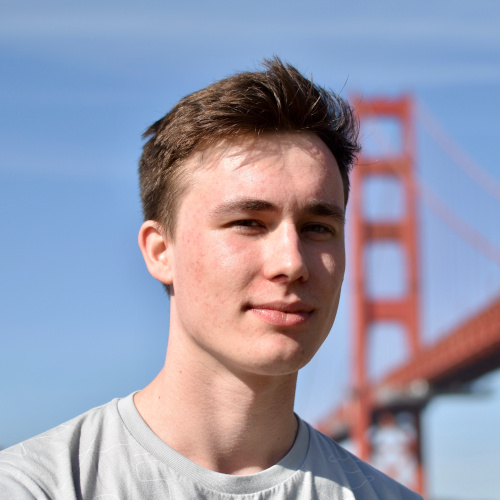
\includegraphics[scale=0.2]{YannHerklotz.jpg}
                \end{figure}
                
            \end{column}


            \begin{column}[]{0.5\textwidth}
                John Wickerson - Lecturer at Dept of Electrical and Electronic Engineering, Imperial College London.
                \begin{figure}
                    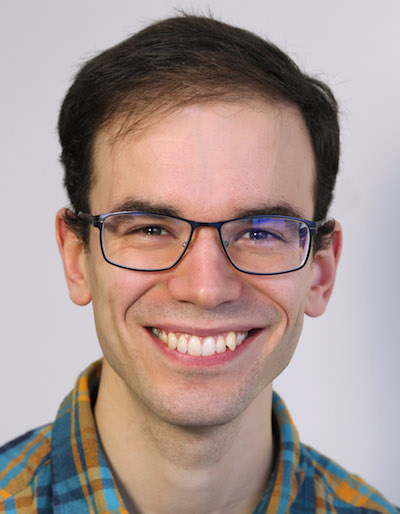
\includegraphics[scale=0.2]{john.jpg}
                \end{figure}
                
            \end{column}



        \end{columns}
        
    \end{frame}


    \logo{}



    \section{Intro}
    \begin{frame}{Introduction: questions}

        \begin{itemize}
            \item What forms of bugs does this paper address? 
            \item Why do they matter? 
            \item How do they address? 
            \item What results did they get?  
        \end{itemize}
        
    \end{frame}

    \subsection{Bugs}
    \begin{frame}{What bugs?}

        \begin{itemize}
            \item Programs are ultimately run by the hardware. 
            \item Circuits are designed today using similar high-level program constructs.
            \item High level synthesis(HLS) tools exist for this purpose. 
            \item If the HLS tools are not designed correctly, can we trust the hardware on which our programs run? 
        \end{itemize}
        
    \end{frame}

    \note{
        Some circuit out there (eg: CPU, GPU, FPGA, ASIC) ultimately runs whatever program we write.
        Including running this pdf viewer for this presentation. 
        We assume that whatever hardware that runs our programs is perfectly built.

        Today's era, even hardware is designed by writing high level programs.
        High level synthesis tools are used to take this program and generate hardware. 
        
        So if the HLS tools are not designed correctly, can we trust the hardware on which our programs run? 

    }

    \begin{frame}{What sort of bugs are addressed?}

        \begin{itemize}
            \item Optimizations in HLS are done to meet several needs such as timing, area, power, etc.
            \item The result after synthesis is a netlist (wires and their interconnection to circuit elements). 
            \item If input program and netlist are not same, this is a bug.
            \item If the HLS tool crashes on a valid program, this is a bug. 
        \end{itemize}
        
    \end{frame}

    \note{
        Sometimes the HLS tool crashes for a given program. 
        If the program is syntactically and semantically correct, the HLS tool should not crash. 
        Even if not, it should raise an error, not crash.
        This is also a bug in HLS tool.         

    }

    \subsection{Bug Detection}
    \begin{frame}{How are the bugs detected?}

        \begin{figure}
            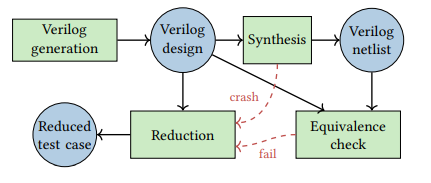
\includegraphics{Verismith_Structure.PNG}
        \end{figure}
        
    \end{frame}

    \note{
        Generate Verilog program via random program generator.
        Give the program to HLS tool to generate netlist. 
        If HLS tool crashes, perform reduction of input program to find out minimal test program to generate the bug. 
        Check equivalence between the netlist and hte program we gave. 
        If they are not equivalent, it is a bug.
        Perform reduction of input program to find out minimal test program to generate the bug.
    }

    \subsection{Result}
    \begin{frame}{What results were obtained?}

        \begin{itemize}
            \item Four tools were tested this way: Yosys, Vivado, XST and Quartus Prime. 
            \item Except Quartus prime(paid version), every other tool had at least one bug of the above types. 
            \item Vivado and Yosys(dev ver.) also crashed for a few program inputs.
        \end{itemize}
        
    \end{frame}

    \section{Main}
    
    \subsection{Code Generation}
    \begin{frame}{Step 1: Program Elements}

        \begin{columns}
            
            \begin{column}[]{0.5\textwidth}
                
                Program elements are:
                \begin{itemize}  
                    \item Modules (line 1..9). 
                    \item Wire (line 2,3,4) and variable (line 5).
                    \item Unary and binary operators (line 8). 
                    \item Assignments (line 6).
                    \item Conditionals (line 8).
                    \item a few more ...     
                \end{itemize}
            \end{column}

            \begin{column}[]{0.5\textwidth}

                \begin{figure}
                    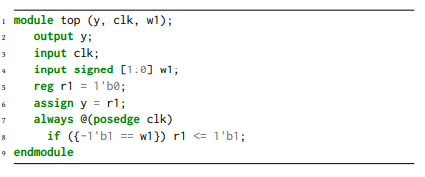
\includegraphics{Elements_Verilog_Deterministic.PNG}
                \end{figure}

            \end{column}

        \end{columns}

    \end{frame}

    \begin{frame}{Step 2: Property of Verilog Programs generated}

        Each Verilog program is 
        \begin{itemize}
            \item Syntactically correct if the HLS tool doesn't complain. 
            \item Semantically correct if the HLS tool doesn't complain. 
            \item Deterministic: they will not have 
                \begin{itemize}
                    \item Divide by zero.
                    \item Wire input from two different sources.
                    \item Using wire not declared previously, etc.
                \end{itemize} 

        \end{itemize}

    \end{frame}

    \begin{frame}{Step 3: Generating Verilog program}

        Programs are generated as follows
        \begin{itemize}
            \item Program elements assigned a frequency (modules, assigns, conditionals, etc).
            \item Context is list of: wire/var assigned, safe modules that can be created, parameters available for module, etc.
            \item Program is built sequentially using context, and updating context after each element addition.
        \end{itemize}

        Output is declared to be a concatenation of all the wire/vars used in the program. 

    \end{frame}

    \subsection{Equivalence}
    \begin{frame}{Step 1: Equivalence Definition}

        Equivalence is defined as:
        \center{\textit{The output wires of the randomly generated verilog program and the netlist synthesized for it should be equal at the clock edge given the same inputs.}} 

        \begin{figure}
            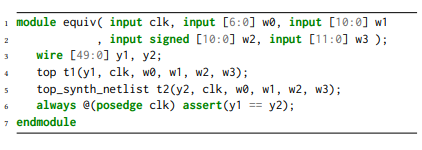
\includegraphics{Equivalence_Code.PNG}
        \end{figure}

    \end{frame}

    \begin{frame}{Step 2: Equivalence Checking}

        \begin{itemize} 
            \item Feed it to Yosys (HLS tool).
            \item Pass it to SMT solver or ABC tool. 
            \item If it returns some result:
                \begin{itemize}
                    \item If a counter example, pass it to reduction phase.
                    \item If no counter example, continue to next verilog design.
                \end{itemize}.
            \item If it timeouts cant do a thing.
        \end{itemize}

    \end{frame}
    

    \subsection{Reduction}
    
    \begin{frame}{Step 1: Reduction Strategy}

        Every reduction step does the following:
        \begin{itemize}
            \item Randomly choose half the modules from the code and remove them. 
            \item Following this, remove half the items of remaining modules (var/nets).
            \item Finally, also remove half the statements(assignments/conditionals) from blocks of code.
            \item Lastly, half the expressions everywhere.
        \end{itemize}

    \end{frame}

    \begin{frame}{Step 2: Reduction halt}

        \begin{itemize}
            \item Reduction is done in a binary fashion. 
            \item Rerun the equivalence checking after every reduction step.
            \item The reduction process is halted when the program no longer produces a bug.
        \end{itemize}
        
    \end{frame}

    \begin{frame}{Step 3: Additional optimization to reduction process}

        Notice that
        \begin{itemize}
            \item Output is a concatenation of all the vars/nets assigned. 
            \item The binary search could be done using only the output. 
            \item Remove half the var/nets associated with output, followed by removing code associated with them. 
        \end{itemize}
        
    \end{frame}


    \subsection{Evaluation}
    \begin{frame}{What do we want to evaluate}
        
        Evaluation is to answer 5 key questions.
        \begin{itemize}
            \item How many unique bugs were detected?
            \item Does bug finding become better as test code size increases?
            \item How does Xor-ing all outputs affect the bug finding process?
            \item How is the stability of synthesis tools across different release versions? 
            \item How does the reduction algorithm of verismith fare with that of Csmith?
        \end{itemize}

        We will look at the first 3 in this presentation.

    \end{frame}


    \begin{frame}{Unique Bug 1}
        
        Yosys peephole optimization.
        \begin{figure}
            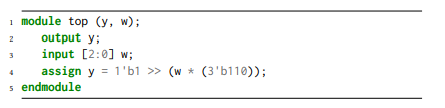
\includegraphics[scale=0.8]{Yosys_Peephole.PNG}
        \end{figure}

        For input like $w=3'b100$, the shift amount is incorrectly given as $6'b011000$, making $y$ $0$.

    \end{frame}

    \note{
            \begin{itemize}
                \item Line 4 is optimized noting that the shift and product contains a constant.
                \item So it can be optimized to $w >> 1 + w >> 2$.
                \item However, proper truncation was not done (note that the product is between 3 bit binaries) 
                \item So the program after optimization, for an input like $w=3'b100$ gave output of $y$ as $0$, instead of $1$.
            \end{itemize}

    }

    \begin{frame}{Unique Bug 2}
        
        Vivado bug.
        \begin{figure}
            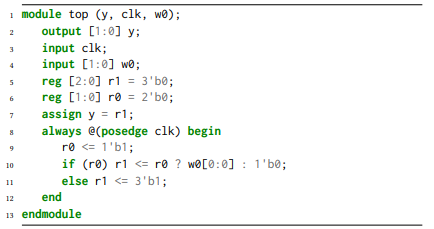
\includegraphics[scale=0.8]{Vivado.PNG}
        \end{figure}

        Line 10 is optimized to have r1 be w[0:0] in 2nd clock cycle.
        However, truncation is not done. So $r1$ is incorrectly a 2-bit value (as opposed to 1-bit).

    \end{frame}

    \note{
        \begin{itemize}
            \item Note that in first clock cycle, Line 11 sets r0 to 1.
            \item Now in the second Clock cycle, Line 12 will always set r1 to w[0:0].
            \item However, this optimization forgets truncation, thus assigning r1 to w.
            \item So when for instance $w=2'b10$, $r1$ is incorrectly $2'b10$ instead of $1'b0$.
        \end{itemize}
    }

    
    \begin{frame}{Summary of Testing}
        
        \begin{figure}
            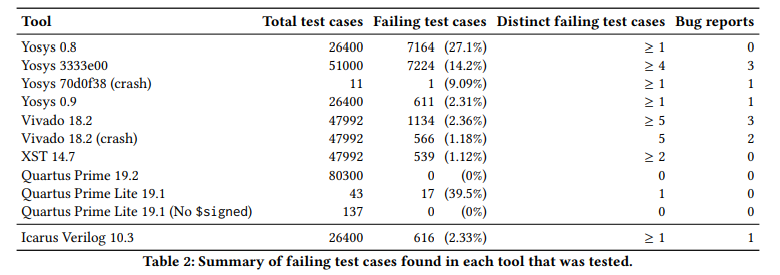
\includegraphics[scale=0.6]{Test_Summary.PNG}
        \end{figure}

    \end{frame}

    \begin{frame}{Code size ?? Bug finding}
        
        Code size vs bug finding, stats. 
        \begin{figure}
            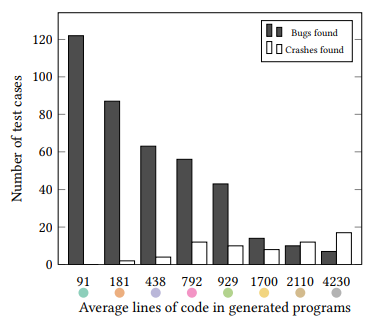
\includegraphics[scale=0.8]{CodeSize_vs_Bugs.PNG}
        \end{figure}

    \end{frame}

    \note{
        \begin{itemize}
            \item The columns from left to right represent how many bugs found for each configuration of verismith.
            \item Configuration was in terms of how many lines of code a test case must contain (with the leftmost being the least).
            \item Interesting to note that the fewer lines of code, the more bugs were uncovered.
            \item However, the bigger the lines of code, the more crashes were identified. 
        \end{itemize}
    }


    \begin{frame}{Xor-ing }
        
        Stats. 
        \begin{figure}
            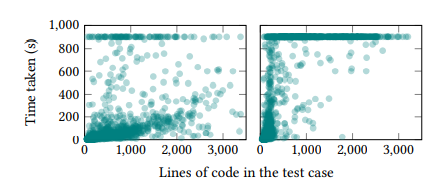
\includegraphics[scale=0.8]{Concat_vs_Xor.PNG}
        \end{figure}
        Bug finding time  worse if we Xor outputs. 
        Counter intuitive.

    \end{frame}

    \note{
        \begin{itemize}
            \item Each chart represents how much time the equivalence check took given lines of code.
            \item The left chart is that when output is a concatenation.
            \item Whereas the right is that when it is a XOR. 
            \item Interesting to note that when the output is XOR, the equivalence checking takes way longer and 1/3rd of the time times out.
            \item Reason can be intuitively viewed as: Xor-ing introduces another set of dependency to output.
            \item So because of this the solver needs to explore more space.
        \end{itemize}
    }

    \section{Discussion}
    \subsection{Pros}
    \begin{frame}{Pros?}
        
        \begin{itemize}
            \item Bugs exist in HLS tools too. :)
            \item Reduction of programs that crash HLS tools. 
            \item Exposing that optimization is also a problem for correctness at synthesis level. 
            \item Equivalence definition using output as a concatenation of vars/nets assigned. 
        \end{itemize}

    \end{frame}

    \subsection{Cons}
    \begin{frame}{Cons?}
        
        \begin{itemize}
            \item Cannot identify bugs at syntax and semantic parts of HLS. 
            \item Reduction process halves modules/outputs. 
            \item Does not work for Verilog code based on undefined values. 
            \item Bug examples in paper seem to only circulate around incorrect assignment of array widths after operations. 
        \end{itemize}

    \end{frame}

    \note {
        \begin{itemize}
            \item Perhaps a better way is to build a dependency tree of all vars/nets and remove mostly connected nodes.  
            \item Perhaps the optimizations should not rely on undefined values to be aggressive like C11.
            \item There could be other forms of bugs, but do they detect them too? 
        \end{itemize}
    }

    \begin{frame}{Thank you!}

        Questions?
        
    \end{frame}


\end{document}